\section{Background}\label{sec:chap4 background}

\subsection{Redistricting ensemble sampling}\label{subsec:districting_ensembles}

The idea of using a score-based probability distribution to assess redistricting counterfactual was introduced in $2014$, concurrently by Mattingly and Vaughn~\cite{mattingly2014redistricting} and Fifield et al.~\cite{fifield2015new}.
Tree-based merge-split samplers have quickly emerged as the standard method to draw samples from ensembles of redistricting plans.
In recombination (Recom), one repeatedly merges two adjacent districts, samples a random spanning tree (using Wilson's algorithm via loop-erased random walk), and then cuts an edge to form two new districts that satisfy population balance constraints~\cite{deford2021recombination}.
Since each step produces two entirely new districts from their union, Recom makes relatively global movements comparing to local node flips.
This implies strong empirical mixing properties in practical applications.
It is worth noting that the spanning-tree construction induces an implicit bias toward compact districts~\cite{deford2021recombination}.

A key limitation of vanilla ReCom is that its stationary distribution generally differs from the target measure chosen by the user, e.g., the one proposed in~\cite{mattingly2014redistricting}.
Moreover, using Recom as a Metropolis-Hastings proposal is infeasible because the forward and reverse proposal probabilities are computationally intractable.
The difficulty mainly comes from the fact that a new spanning tree is chosen in each proposal, which drastically increases the number of possible movements.
To address this problem, Metropolized Forest Recom keeps track of spanning forests instead of just partitions, making forward and backward calculations of proposal probabilities viable~\cite{autry2023metropolized}.
Building on this idea, multi-scale merge-split methods further extend the state space to a forest of tree hierarchies, which has improved scaling properties and is useful for handling county constraints~\cite{autry2020multi}.

In contrast to merge-split proposals that completely resamples a pair of districts, Cycle Walk operates directly on spanning forests using cycle-based local updates: it adds an edge to create a cycle and then removes another edge at random to break the cycle~\cite{cyclewalk}.
This produces relatively local moves comparing to the methods discussed earlier.
The resulting chain can be Metropolized to target a user-specified distribution.
In numerical studies, it shows good convergence performance on examples that are challenging for existing Recom-type algorithms.
In this paper, we use Cycle Walk to generate the redistricting plans as input to our computational pipeline.



\subsection{Stratified Sampling}\label{subsec:umbrella_mbar}
Stratified sampling is a variant of importance sampling that was developed in computational chemistry to overcome the inefficiencies of vanilla Monte Carlo methods.
Originally introduced in the work by Torrie and Valleau to compute free-energy differences under the name umbrella sampling~\cite{torrie1977nonphysical}, the method and its many extensions~\cite{kumar1992weighted,shirts2008statistically} are increasingly formalized in modern statistical literature as stratified samplking or stratified MCMC methods~\cite{dinner2018trajectory}.
One core challenge in these type of problems is that the chain rarely cross large free-energy barriers, making it hard to sample complex measures and rare-events~\cite{kastner2011umbrella,kumar1992weighted}.
This challenge closely mirrors the algorithmic bottlenecks when sampling redistricting plans.
It is known that Recom-type algorithms exhibit prohibitively low accepantace rate when the targeting measure deviates from the tree-count measure~\cite{autry2020multi}.
While newer approaches like Cycle Walk~\cite{cyclewalk} shows empirical improvement, convergence on general measures is still relatively slow.

Stratified sampling addresses this by splitting $\pi$ into easier-to-sample distributions $\{\pi_s\}_{s\in\mathcal{S}}$.
To obtain these distributions, we tilt $\pi$ by nonnegative functions $\{\rho_s\}_{s\in\mathcal{S}}$:
\begin{align}
    \pi_s(x):=\frac{1}{z_s}\rho_s(x)\pi(x),
\end{align}
where $z_s$ is the partition function that normalizes $\pi_s$ into a probability distribution.
The functions $\rho_s$ are designed to cover the phase space, including the low-probability regions, while maintaining overlap to allow for communication between different $\pi_s$.
The main challenge for this type of methods is to find the normalization terms $z_s$.
Let $z$ be the vector formed by concatenating $z_s$.
The following fact about $z$ can be verified via straightforward matrix multiplication:
\begin{align}\label{eqn: umbrella fixed point}
    zG(z)=z,\quad\quad G_{s,s'}(z):=\mathbb{E}_{\pi_s}\left[\frac{\rho_{s'}/z_{s}}{\sum_{t}\rho_{t}/z_{t}}\right].
\end{align}
The above implies that $z$ is a left eigenvector of $G(z)$ with eigenvalue one.
This provides a fixed-point iteration approach to solve $z$ by alternating between updating $G$ and evaluating its left eigenvector $z$, which is essentially the basis of the eigenvector method for umbrella sampling (EMUS)~\cite{dinner2020stratification,matthews2018umbrella}.

Alternatively, one can construct stratified sampling from a soft assignment viewpoint, which forms a more general mathematical framework that easily extends to nonequilibrium sampling~\cite{dinner2018trajectory}.
Suppose we have a set of strata $\mathcal{S}$ equipped with a partition of unity (POU) on the phase space $\{\phi_s\}_{s\in \mathcal{S}}$, which can be viewed as a type of ``soft assignment'' to the strata.
A common way to obtain a set of POU is to start with functions $\psi_s(x)$ and normalize them:
    \begin{align}
        \phi_s(x):=\frac{\psi_s(x)}{\sum_{s\in\mathcal{S}}\psi_s(x)},\quad\quad x\in X.
    \end{align}
This computation is tractable as long as each $x$ is only in the support of $\psi_s$ for a small number of $s$.
Using the POU, we can define stratum weights and a flux matrix via
    \begin{align}
        z_s:=\mathbb{E}_\pi[\phi_s],\quad\quad F_{s,s'}:=\mathbb{E}_{\pi_s}[\phi_{s'}].
    \end{align}
Note that expanding $F_{s,s'}$ using $\phi_s$ gives us an equation that is similar to \eqref{eqn: umbrella fixed point}.
However, the flux matrix $F$ constructed in this way is row-stochastic, whereas $G$ is not in general.
One advantage of using this POU approach is that we can view it as the transition kernel of a Markov chain on the set of strata.



\subsection{Hierarchical clustering}\label{subsec:hierarchical_clustering}
Note that the space of redistricting plans is complex, hence it is generally hard to define meaningful strata.
To address this, we analyze the space of individual districts using hierarchical clustering.
Let $\mathcal{X}=\{x_1,x_2,\dots x_N\}$ be a dataset of size $N$, and $D\in\mathbb{R}^{N\times N}$ be the pairwise distances.
A hierarchical clustering algorithm maps $D$ to an ultrametric distance matrix $D_T$.
The resulting output of a hierarchical clustering algorithm can be viewed in several mathematically equivalent ways: a nested sequence of partitions on $\mathcal{X}$, a binary tree with $N$ leaves (a dendrogram), or an ultrametric topology on $\mathcal{X}$~\cite{murtagh2012algorithms}. 

The nodes of a dendrogram are subsets of $\mathcal{X}$, which can also be viewed as clusters of data points.
In a dendrogram, singleton leaves $\{x_i\}$ gradually merge until they form the root $\mathcal{X}$.
By construction, any two nodes within a dendrogram are either completely disjoint, or one is entirely contained within the other.
The vertical axis of a dendrogram represents the ultrametric distance, a metric that satisfies the strong triangle inequality:
    \begin{align}
        d(x_i,x_j)\leq\max(d(x_i,x_k),d(x_j,x_k)),\quad\quad x_i,x_j,x_k\in\mathcal{X}.
    \end{align}
This condition implies that the distance between any two leaves is simply the height of their lowest common ancestor in the dendrogram.
To extract a clustering of size $K$, one simply ``cuts'' the dendrogram at a specific threshold.
In other words, we discard the edges above the threshold, allowing the sub-trees below the threshold to form a size-$K$ partition of $\mathcal{X}$.
See Figure \ref{fig:dendro_example} for an example of a dendrogram, as well as the cutting procedure.
\begin{figure}[!htbp]
    \centering
    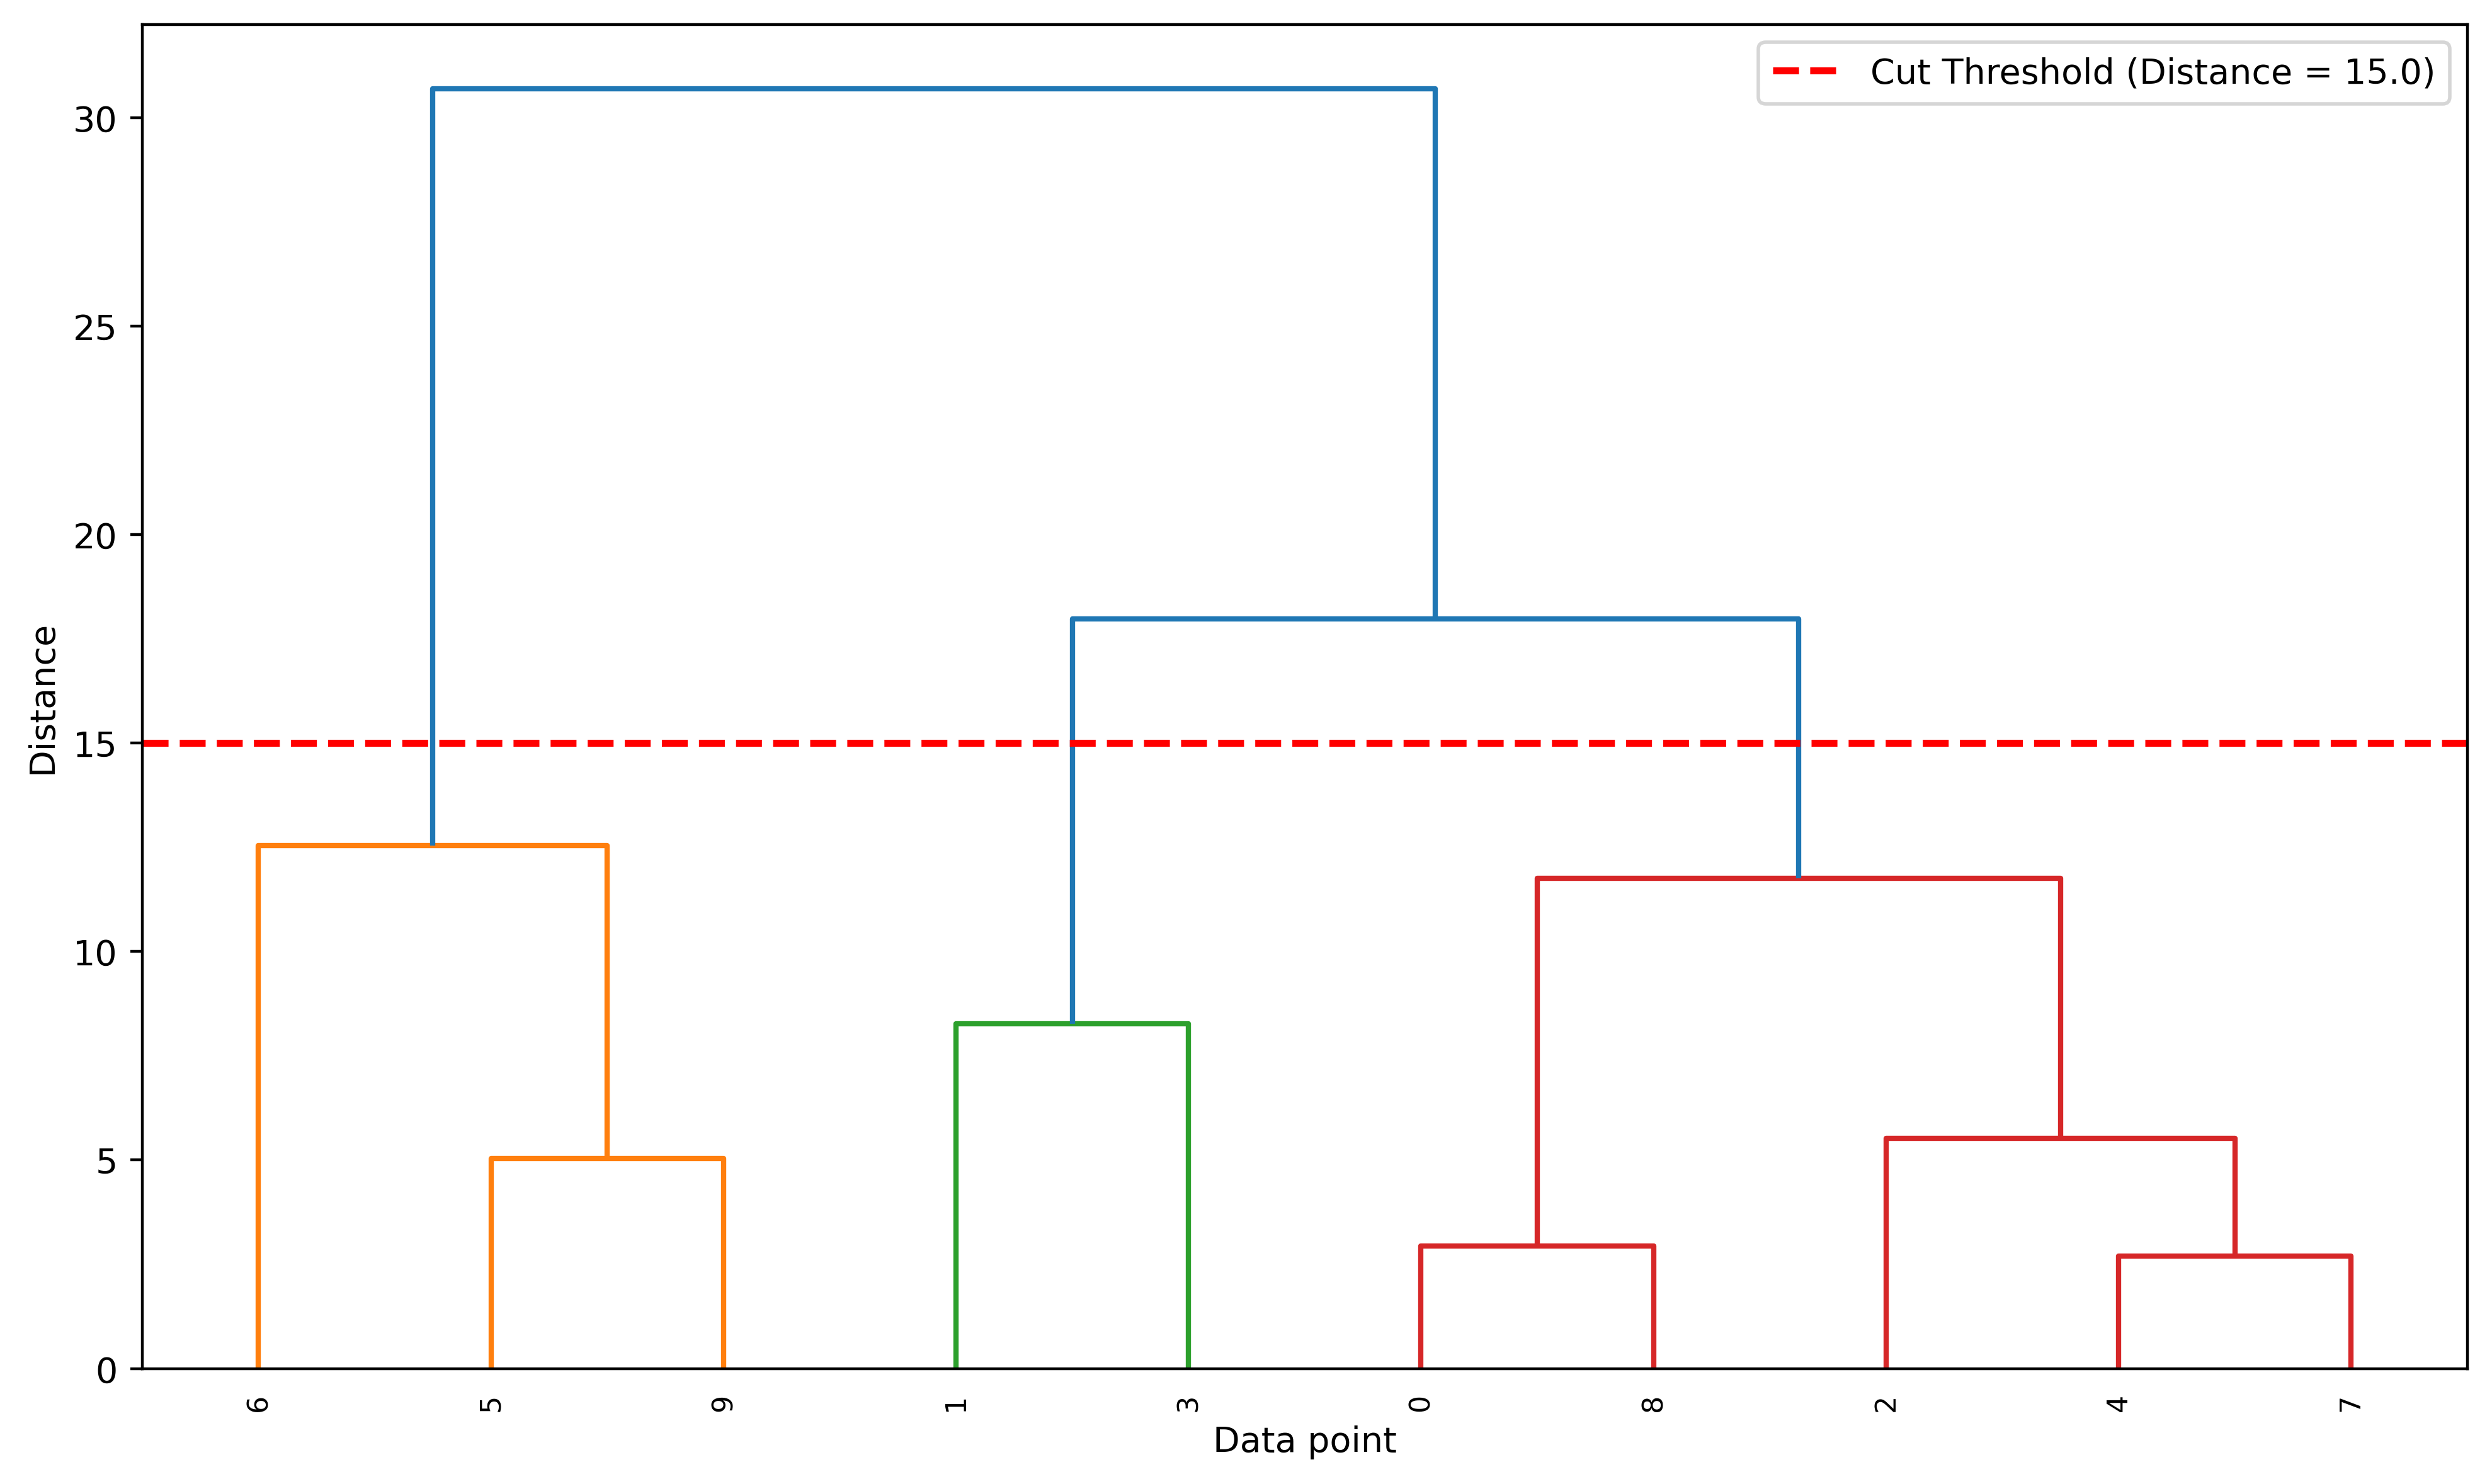
\includegraphics[width=0.8\linewidth]{figures/dendro_example.png}
    \caption{Example dendrogram: $x$-axis shows the indices of data points ($10$ in total), $y$- axis shows the ultrametric distance. The red dashed line indicates a cut at distance $15$, producing three clusters (colored in orange, green and red).}
    \label{fig:dendro_example}
\end{figure}

Classical strategies for building the dendrogram typically involve greedy and irreversible steps that merge the closest pair of clusters at each step based on a heuristic linkage criterion (e.g., single, complete or average linkage)~\cite{sibson1973slink,defays1977efficient,sokal1958statistical}.
While these linkage criteria are easy to implement, they typically do not capture the underlying geometry of the dataset due to their heuristic nature, i.e., ultrametric induced by the dendrogram may be far from the original distances.
In contrast, \hccultra~\cite{DBLP:journals/corr/abs-2409-01010} addresses this problem by proposing a hierarchical correlation clustering algorithm. 
This method fits an ultrametric to $\mathcal{X}$ with a theoretical guarantee on the number of disagreement pairs across every partition level. 
Such consistency across the hierarchy is not observed in common linkage based methods. 
Although the primary goal of \hccultra in~\cite{DBLP:journals/corr/abs-2409-01010} is to manage ultrametric distances, our computational pipeline specifically utilizes their implementation to generate district clusters. Note that we only use the dendrogram output of \hccultra, but the original paper~\cite{DBLP:journals/corr/abs-2409-01010} has a much wider scope.
